%%%%%%%%%%%%%%%%%%%%%%%%%%%%%%%%%%%%%%%%%%%%%%%%%%%%%%%%%%%%%%%%%%%%%%%%%%%
%% This file is part of the book
%%
%% Algorithmic Graph Theory
%% http://code.google.com/p/graph-theory-algorithms-book/
%%
%% Copyright (C) 2009, 2010, 2011 Minh Van Nguyen <nguyenminh2@gmail.com>
%%
%% See the file COPYING for copying conditions.
%%%%%%%%%%%%%%%%%%%%%%%%%%%%%%%%%%%%%%%%%%%%%%%%%%%%%%%%%%%%%%%%%%%%%%%%%%%

\documentclass{article}

\usepackage{subfigure}
\usepackage{tikz}
\usetikzlibrary{external}
\usetikzlibrary{trees}
\tikzexternalize{Fibonacci-trees}

\newcommand{\cF}{\mathcal{F}}

\begin{document}

\begin{figure}
\subfigure[$\cF_0$]{

\begin{tikzpicture}
[-,thick,%
  nodeDecorate/.style={shape=circle,inner sep=2pt,draw,thick},%
  scale=0.5]
%% nodes or vertices
\node at (0,0) [nodeDecorate] {};
%% stub nodes that should not be visible
\node at (-0.5,0) {};
\node at (0.5,0) {};
\end{tikzpicture}
}
%%
%%
\qquad
\subfigure[$\cF_1$]{

\begin{tikzpicture}
[-,thick,%
  every node/.style={shape=circle,inner sep=2pt},%
  scale=0.5]
\node[draw,thick] {}
  [sibling distance=1cm]
  child {node[draw,thick] {}}
  child {node[draw,thick] {}};
%% stub nodes that should not be visible
\node at (-0.6,0) {};
\node at (0.6,0) {};
\end{tikzpicture}
}
%%
%%
\qquad
\subfigure[$\cF_2$]{
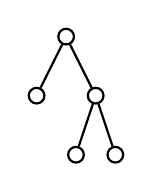
\begin{tikzpicture}
[-,thick,%
  every node/.style={shape=circle,inner sep=2pt,draw,thick},%
  scale=0.5]
\node {}
  child {node {}}
  child {node {}
    [sibling distance=1cm]
    child {node {}}
    child {node {}}
  };
\end{tikzpicture}
}
%%
%%
\qquad
\subfigure[$\cF_3$]{
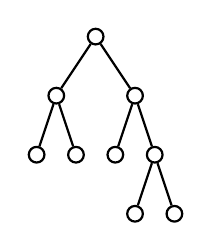
\begin{tikzpicture}
[-,thick,%
  every node/.style={shape=circle,inner sep=2pt,draw,thick},%
  scale=0.5]
\node {}
  [sibling distance=2cm]
  child {node {}
    [sibling distance=1cm]
    child {node {}}
    child {node {}}
  }
  child {node {}
    [sibling distance=1cm]
    child {node {}}
    child {node {}
      child {node {}}
      child {node {}}
    }
  };
\end{tikzpicture}
}
%%
%%
\qquad
\subfigure[$\cF_4$]{
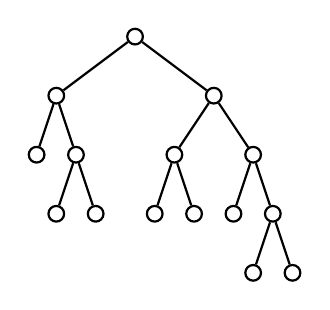
\begin{tikzpicture}
[-,thick,%
  every node/.style={shape=circle,inner sep=2pt,draw,thick},%
  scale=0.5]
\node {}
  [sibling distance=4cm]
  child {node {}
    [sibling distance=1cm]
    child {node {}}
    child {node {}
      child {node {}}
      child {node {}}
    }
  }
  child {node {}
    [sibling distance=2cm]
    child {node {}
      [sibling distance=1cm]
      child {node {}}
      child {node {}}
    }
    child {node {}
      [sibling distance=1cm]
      child {node {}}
      child {node {}
        child {node {}}
        child {node {}}
      }
    }
  };
\end{tikzpicture}
}
%%
%%
\qquad
\subfigure[$\cF_5$]{
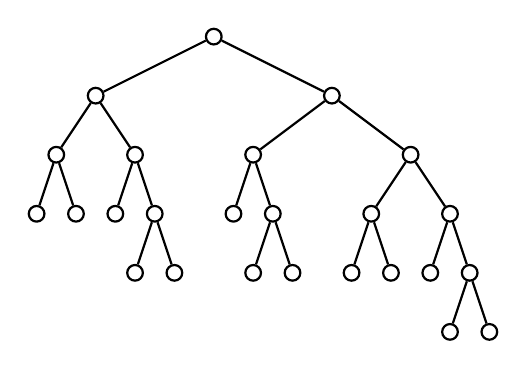
\begin{tikzpicture}
[-,thick,%
  every node/.style={shape=circle,inner sep=2pt,draw,thick},%
  scale=0.5]
\node {}
  [sibling distance=6cm]
  child {node {}
    [sibling distance=2cm]
    child {node {}
      [sibling distance=1cm]
      child {node {}}
      child {node {}}
    }
    child {node {}
      [sibling distance=1cm]
      child {node {}}
      child {node {}
        child {node {}}
        child {node {}}
      }
    }
  }
  child {node {}
    [sibling distance=4cm]
    child {node {}
      [sibling distance=1cm]
      child {node {}}
      child {node {}
        child {node {}}
        child {node {}}
      }
    }
    child {node {}
      [sibling distance=2cm]
      child {node {}
        [sibling distance=1cm]
        child {node {}}
        child {node {}}
      }
      child {node {}
        [sibling distance=1cm]
        child {node {}}
        child {node {}
          child {node {}}
          child {node {}}
        }
      }
    }
  };
\end{tikzpicture}
}
\end{figure}

\end{document}
